\todo[color=red]{Das große Problem ist: Wir haben das $U_0$ nicht bestimmt. Ich habe es einfach auf 20 Volt geschätzt. Es scheint jedoch etwas kleiner gewesen zu sein.}

\subsection{Berechnung der Zeitkonstanten durch}
\subsubsection{... die Aufladekurve des Kondensators}
Um die Gleichung für die linerade Regression zu erhalten, wird Formel \eqref{eq:aufladen} umgeformt zu:
\begin{equation}
\ln(U_C - U_0) = -\frac{1}{RC} t + \ln(U_0)
\end{equation}
Die angelegte Spannung $U_0$ entspricht der Peak to Peak Amplitude der Rechteckspannung.
\begin{align*}
	U_0 = \SI{20}{\volt}
\end{align*}
In Abbildung \ref{fig:spannung1} ist die Differenz der angelegten Spannung und der Kondensatorspannung $U_0 - U_C$ halblogarithmisch über die Zeit aufgetragen. Eine lineare Ausgleichsrechnung der Form
\begin{equation}
\ln(U_C - U_0) = m \cdot t + b
\end{equation} an die in Tabelle \ref{tab:aufladekurve} dargestellten Werte mittels Python liefert:
\begin{align}
	m = \SI{-964.0(229)}{\second} \\
	b = \num{2.84(4)} \\
	\text{Zeitkonstante:} \quad RC = - \frac{1}{m} = \SI{1,037(25)e-3}{\second} \\
	\text{Berechnete Ausgangsspannung:} \quad U_{0\text{reg}} = e ^b \, \si{\volt} = \SI{17,1(6)}{\volt}
\end{align}
	
	
	
	
	

\begin{figure}[h!]
	\centering
	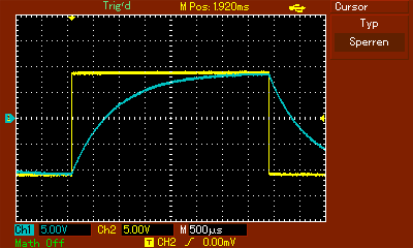
\includegraphics[width=0.7\textwidth]{aufladekurve.png}
	\caption{Aufladekurve des Kondensators bei angelegter Rechteckspannung}
	\label{fig:aufladekurve}
\end{figure} 

\begin{figure}[h!]
	\centering
	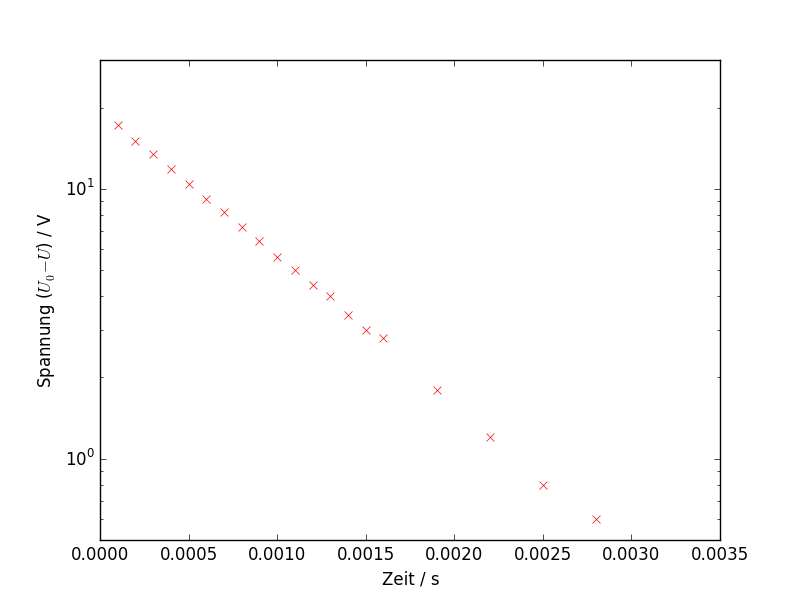
\includegraphics[width=0.7\textwidth]{Spannung1.png}
	\caption{Spannungsdifferenzen halblogarithmisch aufgetragen}
	\label{fig:spannung1}
\end{figure} 

\begin{figure}[h!]
	\centering
	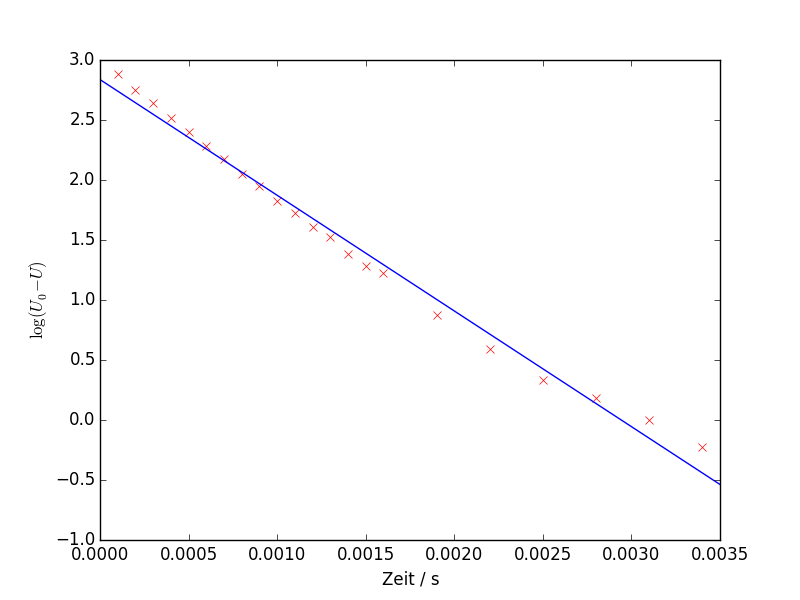
\includegraphics[width=0.7\textwidth]{Spannung2.png}
	\caption{Ausgleichsgerade zur Bestimmung der Zeitkonstanten}
	\label{fig:Spannung2}
\end{figure} 

\begin{figure}[h!]
	\centering
	\captionof{table}{Werte der Aufladekurve}
	\begin{tabular}{c|c}
		Zeit in \si{\milli\second}& $\ln(U_0-U)$ \\
		\hline
		0.1 &  2.88 \\
		0.2 &  2.75 \\
		0.3 &  2.64 \\
		0.4 &  2.52 \\
		0.5 &  2.4  \\
		0.6 &  2.28 \\
		0.7 &  2.17 \\
		0.8 &  2.05 \\
		0.9 &  1.95 \\
		1   &  1.82 \\
		1.1 &  1.72 \\
		1.2 &  1.61 \\
		1.3 &  1.53 \\
		1.4 &  1.39 \\
		1.5 &  1.28 \\
		1.6 &  1.22 \\
		1.9 &  0.88 \\
		2.2 &  0.59 \\
		2.5 &  0.34 \\
		2.8 &  0.18 \\
		3.1 &  0    \\
		3.4 & -0.22 \\
	\end{tabular}
	\label{tab:aufladekurve}
\end{figure}



\clearpage
\subsubsection{... die Ampitude bei periodischer Anregung}
\begin{figure}[h!]
\centering
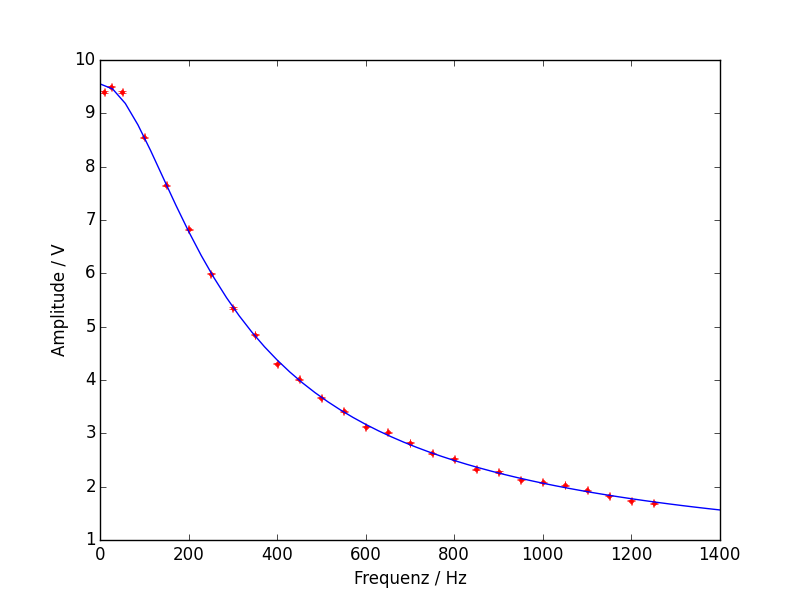
\includegraphics[width=0.7\textwidth]{Amplitude.png}
\caption{Amplitude in Abhängigkeit der Frequenz}
\label{fig:amplitude}
\end{figure} 
